\section{Chandra Kirana Poetra (1174079)}
\subsection{Instalasi Map Server}
\begin{enumerate}
    \item Download aplikasi ms4w melalui website official
    \hfill\break
    \begin{figure}[H]
		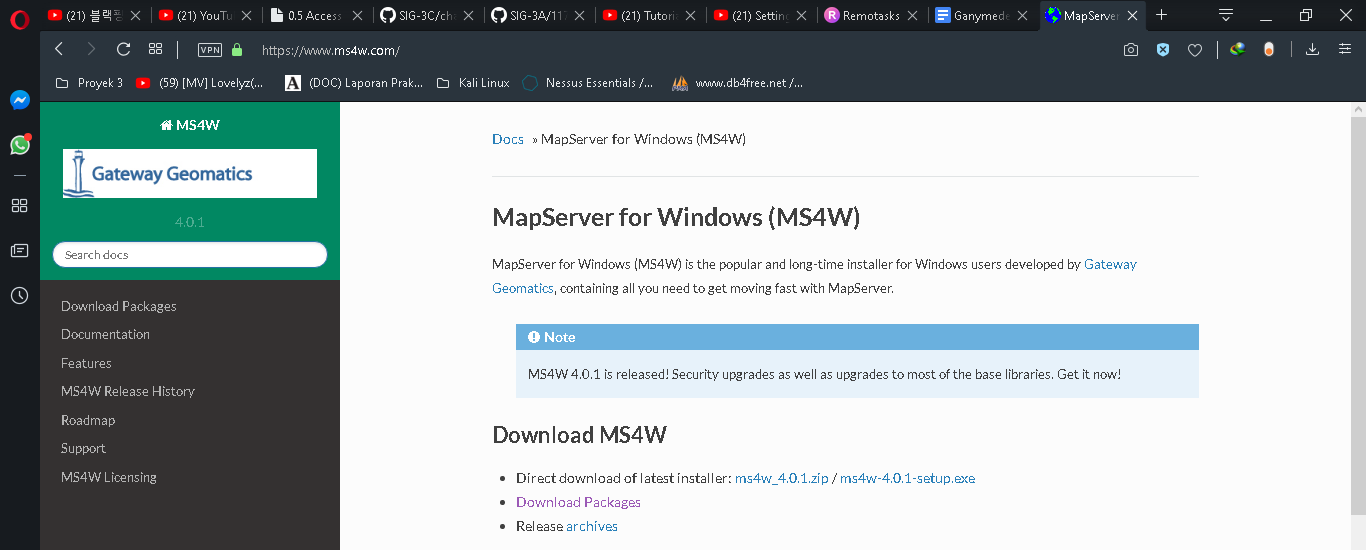
\includegraphics[width=4cm]{figures/tugas4/1174079/1_download_MS4.png}
		\centering
		\caption{Download MS4W}
    \end{figure}
    \hfill\break

    \item Klik Agree
    \hfill\break
    \begin{figure}[H]
		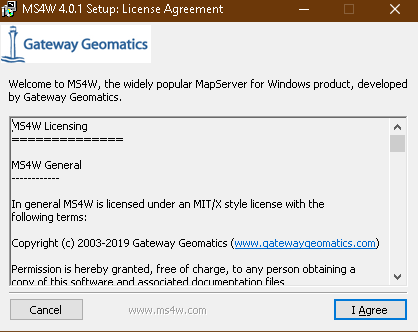
\includegraphics[width=4cm]{figures/tugas4/1174079/2_MS4_Agree.png}
		\centering
		\caption{Download MS4W}
    \end{figure}
    \hfill\break
    \item Pilih opsi Full Install
    \hfill\break
    \begin{figure}[H]
		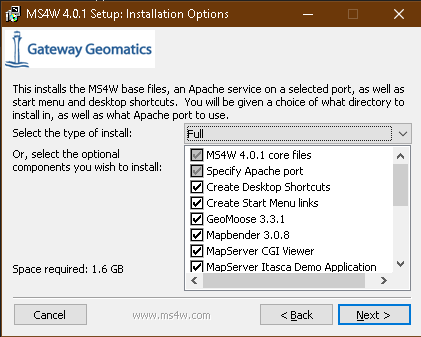
\includegraphics[width=4cm]{figures/tugas4/1174079/3_Full_Install.png}
		\centering
		\caption{Download MS4W}
    \end{figure}
    \hfill\break

\end{enumerate}

\subsection{Konfigurasi Map Server}
Setelah selesai melakukan instalasi kemudian konfigurasikan MS4W nya
\begin{enumerate}
  \item Buka Folder tempat anda install Mapserver4 lalu pergi ke folder ms4w kemudian apache lalu conf
  \hfill\break
    \begin{figure}[H]
		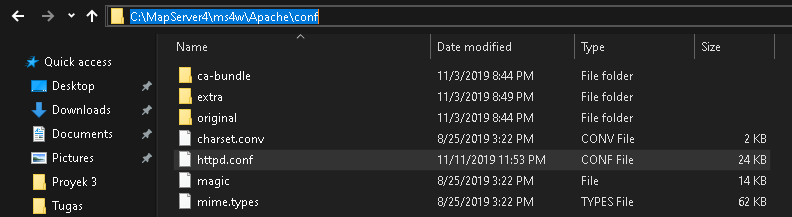
\includegraphics[width=4cm]{figures/tugas4/1174079/4_Konfigurasi_MS4W.png}
		\centering
		\caption{Folder }
    \end{figure}

  \item Buka file httpd.conf menggunakan editor favorit anda lalu ubah menjadi 1000 agar tidak konflik dengan XAMPP jika ada di komputer.
  \hfill\break
    \begin{figure}[H]
		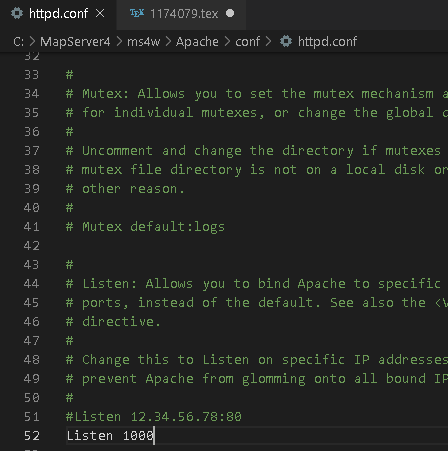
\includegraphics[width=4cm]{figures/tugas4/1174079/5_Port.png}
		\centering
		\caption{File httpd.conf}
    \end{figure}

  \item Jika sudah buka services dengan menggunakan cmd
  \hfill\break
    \begin{figure}[H]
		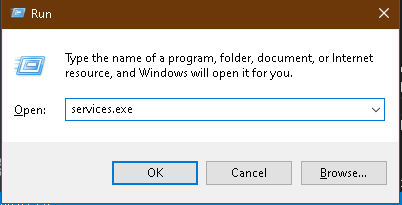
\includegraphics[width=4cm]{figures/tugas4/1174079/6_Buka_Services.png}
		\centering
		\caption{Task Manager}
    \end{figure}

  \item Lalu pilih ApacheMS4WWebServer dan klik restart
  \hfill\break
  \begin{figure}[H]
  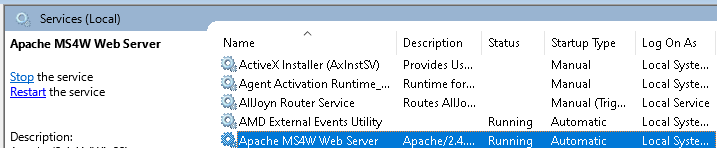
\includegraphics[width=4cm]{figures/tugas4/1174079/7_restart_MS4W.png}
  \centering
  \caption{Pilih tab service dan pilih ApacheMS4WWebServer}
  \end{figure}

\end{enumerate}

\subsection{Link Youtube Instalasi MapServer}
https://youtu.be/FU9tGvKfWqg

\subsection{Instalasi MapProxy}
\begin{enumerate}
  \item Buka CMD
  \item ketik pip install MapProxy
  \hfill\break
  \begin{figure}[H]
  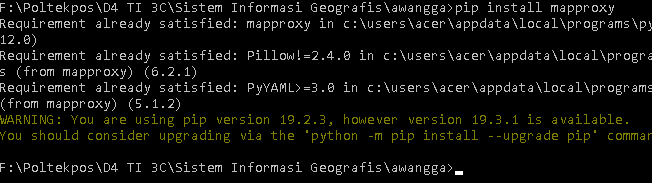
\includegraphics[width=4cm]{figures/tugas4/1174079/mapproxyinstall.png}
  \centering
  \caption{Instalasi MapProxy}
  \end{figure}
\end{enumerate}

\subsection{Membuka map menggunakan MapProxy}
\begin{enumerate}
  \item clone dulu git dari https://github.com/awangga/gede
  \item Pastikan path menuju folder gede tidak ada spasi contoh E:/gede-master
  \item Buat folder bernama tmp di gede-master
  \hfill\break
  \begin{figure}[H]
  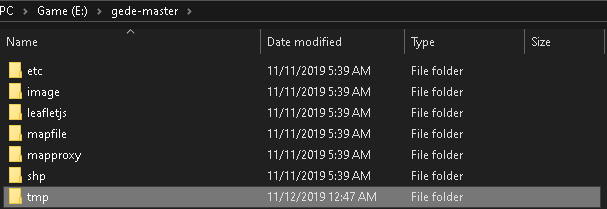
\includegraphics[width=4cm]{figures/tugas4/1174079/8_Pembuatan_Folder_TMP.png}
  \centering
  \caption{Buat folder tmp}
  \end{figure}

  \item kemudian buka folder mapproxy lalu edit file agm.yaml
  \hfill\break
  \begin{figure}[H]
  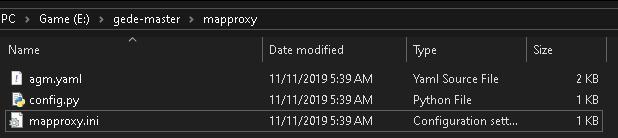
\includegraphics[width=4cm]{figures/tugas4/1174079/9_fileAGM.png}
  \centering
  \caption{File agm.yaml}
  \end{figure}

  \item Pada bagian sources lalu ada map, masukkan pathnya sesuai dengan tempat direktori gede yang anda clone :/gede-master/mapfile/mywms.map
  \hfill\break
  \begin{figure}[H]
  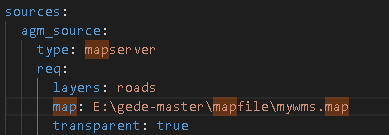
\includegraphics[width=4cm]{figures/tugas4/1174079/10_Edit_AGM.png}
  \centering
  \caption{Edit lokasi mymap.map}
  \end{figure}


  \item Lalu dibawahnya pada bagian binary masukkan lokasi instalasi ms4w anda, lalu tambahkan C:/ms4w/Apache/cgi-bin/mapserv.exe tempat anda install mapserver, bagian working dir juga tambahkan direktori folder tmp
  \hfill\break
  \begin{figure}[H]
  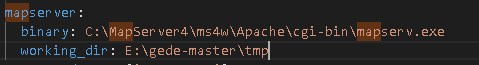
\includegraphics[width=4cm]{figures/tugas4/1174079/11_Edit_AGM.png}
  \centering
  \caption{Edit path binary mapserv}
  \end{figure}

  \item Setelah itu buka aplikasi MS4W-Shell
  \hfill\break
  \begin{figure}[H]
  
\includegraphics[width=4cm]{figures/tugas4/1174079/10.jpg}
  \centering
  \caption{Aplikasi MS4W-Shell}
  \end{figure}

  \item Setelah itu buka lokasi folder gede kita yang tadi telah di clone
  \hfill\break
  \begin{figure}[H]
  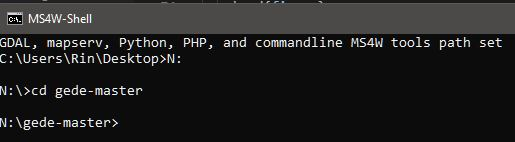
\includegraphics[width=4cm]{figures/tugas4/1174079/12.jpg}
  \centering
  \caption{Buka Folder gede}
  \end{figure}

  \item Setelah itu buka folder mapproxy yang ada pada folder gede
  \hfill\break
  \begin{figure}[H]
  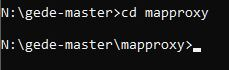
\includegraphics[width=4cm]{figures/tugas4/1174079/17.jpg}
  \centering
  \caption{Buka Folder mapproxy}
  \end{figure}

  \item setelah dibuka ketikkan "mapproxy-util serve-develop ./agm.yaml" pada ms4w-Shell untuk membuka aplikasi mapproxy
  \hfill\break
  \begin{figure}[H]
  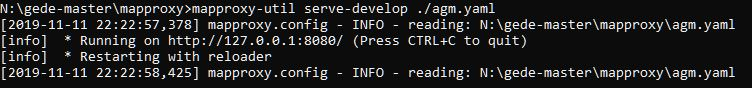
\includegraphics[width=4cm]{figures/tugas4/1174079/18.jpg}
  \centering
  \caption{Buka aplikasi mapproxy}
  \end{figure}
  
  \item Buka browser lalu ketikkan 127.0.0.1:8080
  \hfill\break
  \begin{figure}[H]
  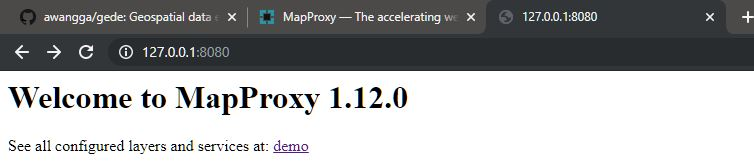
\includegraphics[width=4cm]{figures/tugas4/1174079/19.jpg}
  \centering
  \caption{Buka mapproxy pada browser}
  \end{figure}

  \item lalu klik demo untuk melihat map
  \item lalu klik png pada agm, maka mapproxy akan menampilkan map
  \hfill\break
  \begin{figure}[H]
  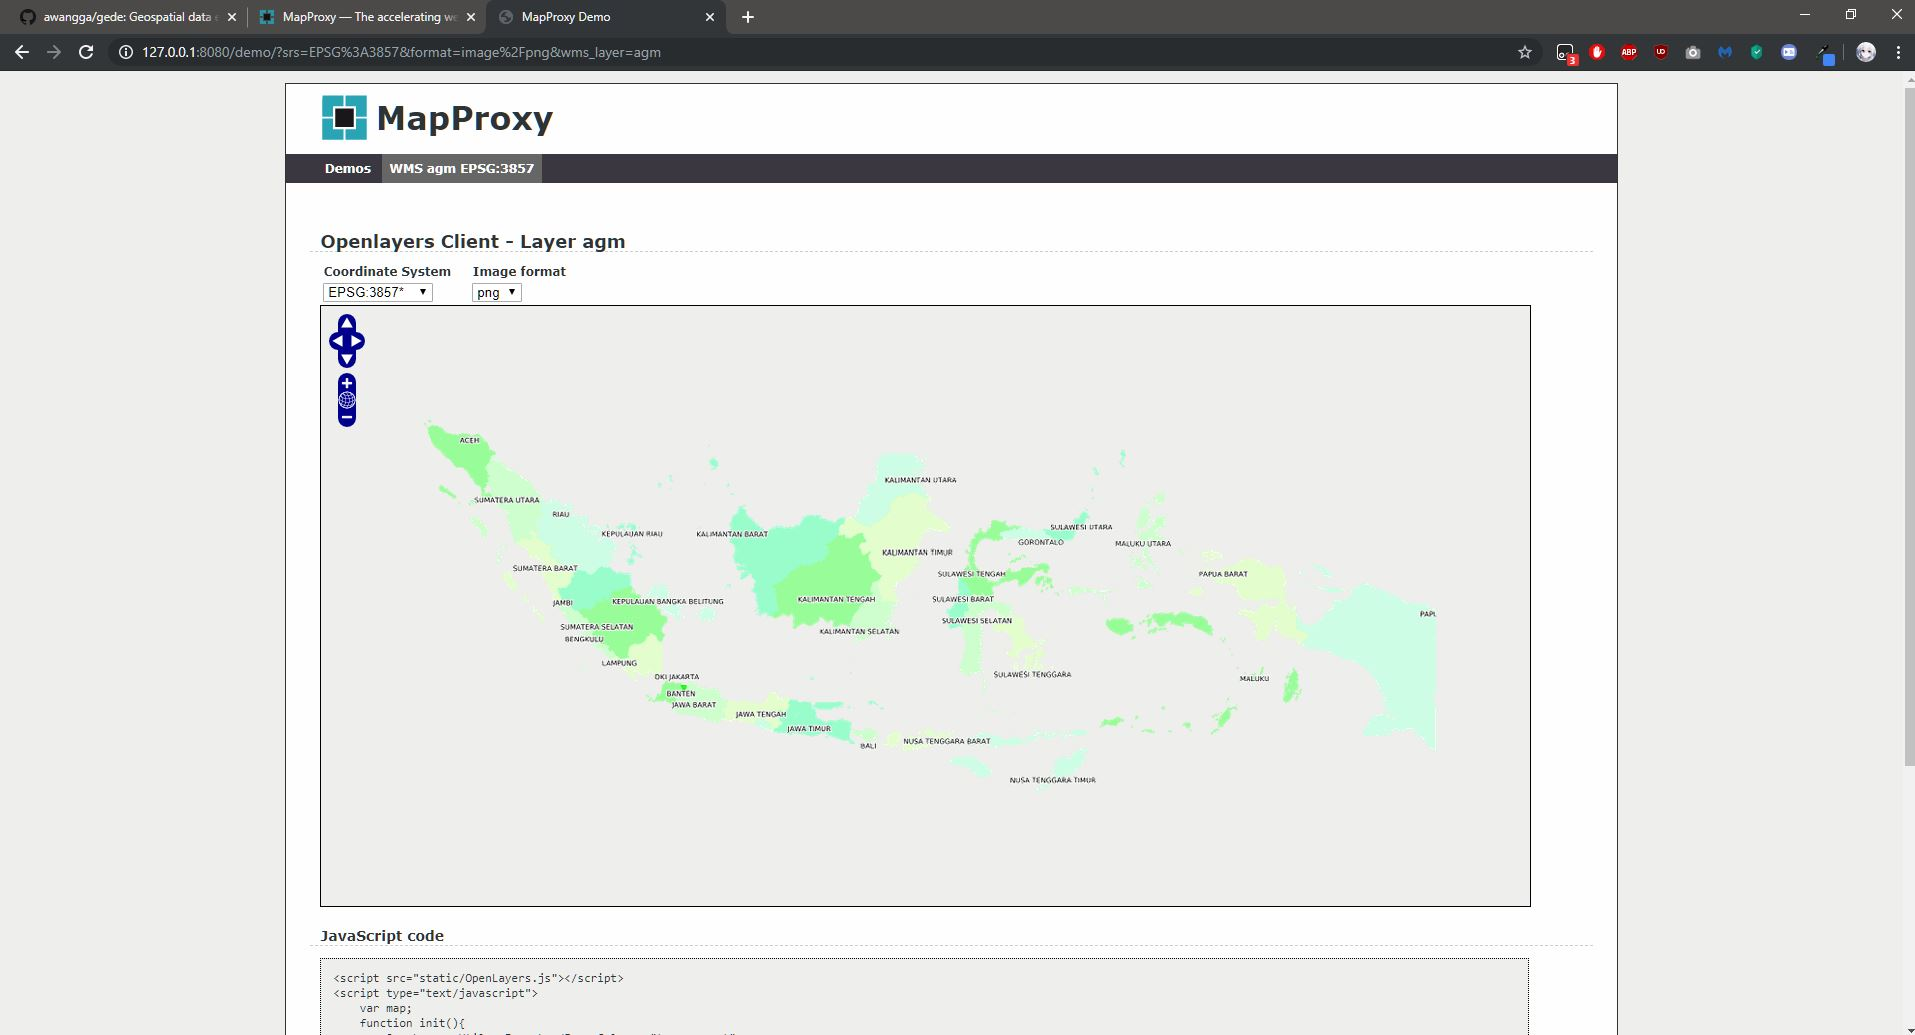
\includegraphics[width=4cm]{figures/tugas4/1174079/20.jpg}
  \centering
  \caption{MapProxy menampilkan map}
  \end{figure}

\end{enumerate}

\subsection{Link Youtube MapProxy dan Menjalankannya}
https://youtu.be/JffJxW4oETE


